\documentclass[a4paper,12pt]{article}

\usepackage{cmap}		
\usepackage[utf8]{inputenc}			
\usepackage[english,russian]{babel}
\usepackage{framed}
\usepackage{hyperref}
\usepackage{amsmath}
\usepackage[colorinlistoftodos]{todonotes}
\usepackage{wrapfig}
\usepackage{lipsum}
\usepackage{listings}
\usepackage{color}
\usepackage{indentfirst}
\usepackage{times}
\usepackage{textcomp}
\usepackage{smartdiagram}
\usepackage{caption}
\usesmartdiagramlibrary{additions}
\usepackage{tikz}
\usepackage{multicol}
\usepackage{lipsum}
\usepackage{mwe}
\usepackage{floatrow}
\usepackage[ruled,linesnumbered,vlined]{algorithm2e}
\usepackage{algpseudocode}
\usepackage[final]{graphicx}
\usepackage{subfigure}
\usepackage{subcaption}
\usepackage{minted}
\usepackage{placeins}
\usepackage{amsfonts}
\usepackage{lscape}
\usepackage{subcaption}
\usepackage{enumitem}
\usepackage{siunitx}
\usepackage{array}
\usepackage{pgfplots}
\pgfplotsset{compat=newest}
\usetikzlibrary{arrows,shapes}
\DeclareMathOperator*{\argmin}{arg\,min}
\DeclareMathOperator*{\argmax}{arg\,max}
\DeclareMathOperator{\E}{\mathbb{E}}
\definecolor{mygray}{rgb}{0.4,0.4,0.4}
\definecolor{mygreen}{rgb}{0,0.8,0.6}
\definecolor{myorange}{rgb}{1.0,0.4,0}


\definecolor{mygray}{rgb}{0.4,0.4,0.4}
\definecolor{mygreen}{rgb}{0,0.8,0.6}
\definecolor{myorange}{rgb}{1.0,0.4,0}

\lstdefinestyle{customc}{
  belowcaptionskip=1\baselineskip,
  breaklines=true,
  frame=L,
  xleftmargin=\parindent,
  language=C,
  showstringspaces=false,
  basicstyle=\footnotesize\ttfamily,
  keywordstyle=\bfseries\color{green!40!black},
  commentstyle=\itshape\color{purple!40!black},
  identifierstyle=\color{blue},
  stringstyle=\color{orange},
  numbers=left,
  numbersep=12pt,
  numberstyle=\small\color{mygray},
}
\lstset{escapechar=@,style=customc}

\newcommand{\HRule}{\rule{\linewidth}{0.5mm}}
\DeclareMathOperator*{\argmax}{arg\,max}
\DeclareMathOperator*{\argmin}{arg\,min}

\begin{document}

\begin{titlepage}
\begin{center}

\textsc{\Large Московский Государственный Технический Университет имени Н.Э.Баумана}\\
\textsc{\large (Национальный Исследовательский Университет)}\\[1.5cm]

% Upper part of the page. The '~' is needed because \\
% only works if a paragraph has started.

\includegraphics[width=0.3\textwidth]{img/logo.png}~\\[1cm]

\textsc{\Large Курсовой проект по проектированию}\\[0.5cm]

% Title
\HRule \\[0.4cm]
{ \LARGE \bfseries Проектирования системы управления на базе обучения с подкреплением\\[0.4cm] }

\HRule \\[1.5cm]

% Author and supervisor
\noindent
\begin{minipage}{0.4\textwidth}
\begin{flushleft} \large
\emph{Студент:}\\
Юнес \textsc{А.~Ю.}
\end{flushleft}
\end{minipage}%
\begin{minipage}{0.4\textwidth}
\begin{flushright} \large
\emph{Рукаводитель:} \\
Ющенко \textsc{А.~С.}
\end{flushright}
\end{minipage}

\vfill

% Bottom of the page
{\large \today}

\end{center}
\end{titlepage}

% \newpage
% \begin{abstract}
    
%     The standard control methods in robotics are based on the dynamical model of the robot, and also on the model of the dynamics of the environment to build the needed closed loop control scheme; in the real world to realize such methods for manipulators, we have to follow the following steps: (1) taking an observation of the environment using cameras or sensors (2) estimating the state of the robot and the task (e.g,position of the end-effector and the goal position) (3) planing the trajectory of motion of the end-effector to achieve the task (4) using low-level controllers (or force controller for harder tasks) to ensure following the planned path by minimizing the errors (5) sending the resulting commands to the joints of the robot. The errors which are occurred in each step, accumulated to produce a cumulative error making the control process hard to realize with desired accuracy.\\ \par
%     We suggest using the machine learning to achieve end-to-end mapping directly from observations to joints' motors commands, exploit the last deep learning revolution in using deep (large) neural networks. The state of the art deep reinforcement learning algorithms, that tried to handle robotic tasks can be classified to two major classes: (1) model-free algorithms: (like TRPO,PPO,DDPG) which can learn to achieve the task after sampling training sets from interacting with environment, so we can consider the robot's model as a black-box (2)model-based algorithms: depends on a known (or learned) transition model of the environment. The model-free algorithms need days of training to learn basic robotic tasks. On the other hand, model-based algorithms can learn much more faster (less than an hour), but can't adapt to unforeseen situation (the learned model is no longer valid).\\ \par
%     We intend in that research to develop a data-efficient model-free algorithm, which can get the benefits of the both classes of deep reinforcement learning algorithms, and learn the assembly task (which is considered as a hard problem in standard robotic control) in a considerable small period of time.
% \end{abstract}
\newpage
\tableofcontents

\newpage
\listoffigures
\listoftables
 
\newpage
\section{Введение}
\subsection{Обучения с подкреплением - от игр к промышленности}
Целью машинного обучения является частичная или полная создания машину, способную учиться аналогично человеку. Основные стандартные типы задач машинного обучения; (1) Обучение с учителем , при котором машина обучается на основе помеченных данных. (2) Обучение без учителя , процесс обучения работает с непомеченными данными и (3) Обучение с подкреплением, когда процесс обучения зависит от проб и ошибок.\\

Технологические достижения последних лет привели к использованию глубоких нейронных сетей в алгоритмах обучения в качестве мозга машины. Забота о лучших способах мышления вызвала некоторые идеи на свет - одной из них было обучение с подкреплением. Глубокое обучение с подкреплением стала трендом, и базом "Искусственного общего интеллекта" (Artificial General Intelligence).\\

В 2015 году команда Google DeepMind опубликовала статью в журнале Nature, представляющую систему, основанную на обучении подкреплению, под названием AlphGO. Эта система победила над чемпионатом мира в игре GO. Такие важный достижения, мотивировала многих исследователей следовать этому направлению исследований. Новые алгоритмы разработаны после этого, сформировали революцию в приложениях обучения с подкреплением.\\
\begin{figure}[H]
    \centering
    \subfigure[Машинное обучение]{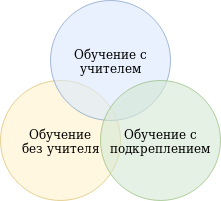
\includegraphics[height=5cm]{img/ML.png}}
    \subfigure[AlphaGO]{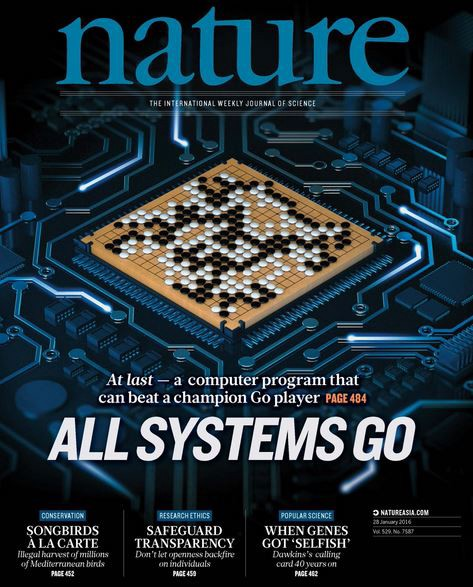
\includegraphics[height=5cm]{img/go.jpeg}}
    \caption{Обучения с подкреплением - от игр к промышленности}
    \label{fig:my_label}
\end{figure}

Но два года позже, в 2017. Опубликовали статью под названием «Глубокое обучение с подкреплением пока не работает», в котором представлен обзор и результаты современных алгоритмов глубокого обучение с подкреплением. Эта статья показала, что еще много работы, чтобы иметь идеальный вариант из алгоритмов обучения с подкреплением.\\

В промышленности интерес заключается в оптимизации процессов производства при сохранении некоторых строгих ограничений. Обучения с подкреплением показало, что он может превзойти человеку и классической управление, когда он работает, поэтому наша цель в этой работе - исследовать различные алгоритмы обучения с подкреплением и обсудить, как мы можем заставить обучение с подкреплением чтобы работать хорошо в реальных промышленных задачах. Попытался предложить практические решения на основе  обучения с подкреплением.\\

\subsection{Актуальность и важность обучения в робототехники}
В области промышленности и робототехники у нас могут быть дополнительные требования к системе наряду с выполнением ее задач. Например, если система космического аппарата с управлением соответствует ракетным двигателям, то целью является достижение Луны с минимальным расходом топлива. 
Оптимальное управление решает такие задачи, ставя своей целью найти закон управления для динамической системы за такой промежуток времени, чтобы целевая функция была оптимизирована; определение набора дифференциальных уравнений, описывающих путь управляющих переменных, которые минимизируют функцию затрат.\\

Модельное прогнозирующее управление (Model predictive control MPC) является одним из популярных методов оптимального управления. MPC был разработан в обществе системы управления, в общем он обеспечивает стабильности, осуществимость и надежности. Кроме того, он может обрабатывать ограничения на систему. Но он основан на динамической модели системы, поэтому на него влияет точность этой модели, и он не может адаптироваться к изменениям и требует высокая вычислительная сложность.\\

С другой стороны, обучение с подкреплением (которое также можно рассматривать как часть оптимального управления) не зависит от модели, способно адаптироваться и имеет низкую вычислительную сложность при развертывании модели после обучения. Но он обладает незрелой стабильностью, осуществимостью и надежностью и трудно обрабатывать ограничения.\\

Мы можем ясно заметить комплементарную связь между модельным прогностическим контролем MPC и обучением с подкреплением, Мы будем в этой работе исследовать, как мы могли бы использовать преимущества обеих парадигм, чтобы получить наилучшие результаты в решении задач управления.

\begin{table}[H]
    \centering
    \captionsetup{justification=centering,margin=1cm}
    \begin{tabular}{| >{\centering\arraybackslash\hspace{0pt}}m{2cm}| >{\centering\arraybackslash\hspace{0pt}}m{5cm}| >{\centering\arraybackslash\hspace{0pt}}m{5cm}|}
         \hline
         Свойство & Модельное прогнозирующее управление & Обучение с подкреплением\\
         \hline
         Модель & Требуемый (-) & Не Требуемый (+)\\
         \hline
         Адаптивность & Зависит от надежность (-) & Присущий (+)\\
         \hline
         Онлайн выч. сложность & Высокая (-)& Низкая (+)\\
         \hline
         Офлайн выч. сложность & Низкая (+) & Высокая (-) \\
         \hline
         Стабильность & Зависит от терминального затрата (+) & Неприсущий(-) \\
         \hline
         Осуществимость & Зависит от терминального ограничения (+) & Неприсущий(-) \\
         \hline
         Надежностью & Присущий (+) & Неприсущий(-) \\
         \hline
         Обработка ограничений & Присущий (+) & Неприсущий(-) \\
         \hline
    \end{tabular}
    \caption{Сравнения  Модельного прогнозирующего управления с Обучением с подкреплением}
    \label{tab:my_label}
\end{table}
\newpage
\section{Постановка задачи}
В обычной модели прогностического регулятора MPC целью является нахождение оптимального управления путем решения задачи оптимизации (оптимизации целевого функционала) по горизонту времени, используя данный модель динамической системы.\\

Мы заинтересованы в использовании модели прогностического управления MPC , когда у нас нет динамической модели системы, а мы будем обучать модель и планировать в ней.\\

Вместо обучения динамическую модель явно, мы будем рассматривать систему как систему Марковского процесса принятия решений (аналогично случаю в обучении подкреплению).\\

Полный алгоритм можно рассматривать как основанную на модели задачу обучения подкреплению, с моделью прогностического регулятора в качестве планировщика. Или проблема модели прогностического управления на основе обучения с подкреплением.\\

\begin{figure}[H]
    \centering
    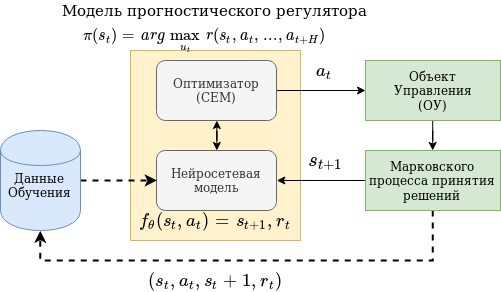
\includegraphics[height=8cm]{img/MPC_ru.png}
    \caption{MPC на основе обучения с подкреплением}
    \label{fig:my_label}
\end{figure}
\newpage
\section{Исследовательская часть} 
\subsection{Оптимальное управления}
\subsubsection{Модель системы и функция стоимости:}
рассмотрим дискретной линейной стационарной системы
\begin{equation}
    x(t+1)=Ax(t)+Bu(t)
\end{equation}
где $x \in \mathbb{R}^n$-вектор состояния, $u \in \mathbb{R}^m$-входной управляющий вектор, $A \in \mathbb{R}^{n \times n}$-системная матрица, $B \in \mathbb{R}^{n \times m}$-входная матрица, $t \in \mathbb{N}$-дискретное время. A и B считаются стабилизированными.\\

Пусть $x(t)$ будет вектор состояния, измеренная в момент времени $t$ и $x_{t+k}$ вектора состояния предсказан в дискретном времени $t+k$, используя уравнение состояния (1) с начальным условием $x_t=x(t)$.//

$x(t)$ и $u(t)$ ограничены из многогранных множеств.\\

Рассмотрим функциал стоимости:
\begin{equation}
    V_N(x(t))=r_T(x_{t+N},u_{t+N})+\sum_{k=0}^{N-1} \gamma^k r(x_{t+k},u_{t+k})
\end{equation}
с стоимость шага:
$$r(x_{t+k},u_{t+k})=x_{t+k}^k Q x_{t+k} + u_{t+k}^T R u_{t+k}$$
и терминальная стоимость:
$$r(x_{t+N},u_{t+N})=x_{t+k}^k P x_{t+k}$$
где $N$-горизонт прогнозирования, $\gamma$-коэффициент дисконтирования,$Q$ состояние весовой матрицы, $R$ входной весовой матрицы и $P$ терминал весовой матрицы.\\

Терминальные матрицы считаются симметричными и положительно определенными.
В качестве решения алгебраического уравнения Риккати выбрана терминальная весовая матрица:
\begin{equation}
    (A+BK)^T P (A+BK)-P+Q+K^T R K=0
\end{equation}
причем :
$$K=-(R+B^T P B)^{-1} B^T P A$$
\subsubsection{Задача Оптимального Управления Конечным Горизонтом}
Оптимизация Функциала:
\begin{equation}
    U_{N}^*(x(t))=\argmin_{U(t)} r_T(x_{t+N},u_{t+N})+\sum_{k=0}^{N-1} \gamma^k r(x_{t+k},u_{t+k})
\end{equation}

\begin{subequations}
C ограничениями:
\begin{align}
    x_{t+k+1} & = Ax_{t+k}+Bu_{t+k}  & k&=0,..,N-1 \\
    x_{t+k} & \in \mathbb{X}  & k&=0,..,N \\
    u_{t+k} & \in \mathbb{U}  & k&=0,..,N-1 \\
    x_t&=x(t) \\
    U(t)&=(u_t^T, ... , u_{t+N-1}^T)^T \in \mathbb{R}^{N_m}
\end{align}
\end{subequations}
Где (5a)- уравнения системы, (5b) - ограничения состоянии, \\ 
\null \qquad (5c) - ограничения управления, (5d) - начальная условия, \\ 
\null \qquad (5e) - управляющая последовательность
\subsubsection{Задача Оптимального Управления Бесконечным Горизонтом}
Оптимизация Функциала:
\begin{equation}
    U_\infty^*(x(t))=\argmin_{U(t)} \sum_{k=0}^{\infty} \gamma^k r(x_{t+k},u_{t+k})
\end{equation}
\begin{subequations}
C ограничениями:
\begin{align}
    x_{t+k+1} & = Ax_{t+k}+Bu_{t+k}  & k&=0,1,.. \\
    x_{t+k} & \in \mathbb{X}  & k&=0,1,.. \\
    u_{t+k} & \in \mathbb{U}  & k&=0,1,.. \\
    x_t&=x(t) \\
    U(t)&=(u_t^T, u_{t+1}^T, ....)^T
\end{align}
\end{subequations}
Где (7a)- уравнения системы, (7b) - ограничения состоянии, \\ 
\null \qquad (7c) - ограничения управления, (7d) - начальная условия, \\ 
\null \qquad (7e) - управляющая последовательность
\newpage
\subsection{Модельное прогнозирующее управление\\
Model Predictive Control (MPC)}
Модельное прогнозирующее управление основано на решении задачи оптимального управления (конечным или бесконечным горизонтом) для измеряемого вектора состояния $x (t)$ с целью получения оптимальной управляющей последовательности $U(t)$ и применения первого элемента оптимальной управляющей последовательности $u(t)=[I,0,..,0] U(t)$ к системе.\\
Эта операция повторяется на каждом дискретном временном шаге t с отступающим горизонтом прогнозирования.\\
\begin{figure}[H]
    \centering
    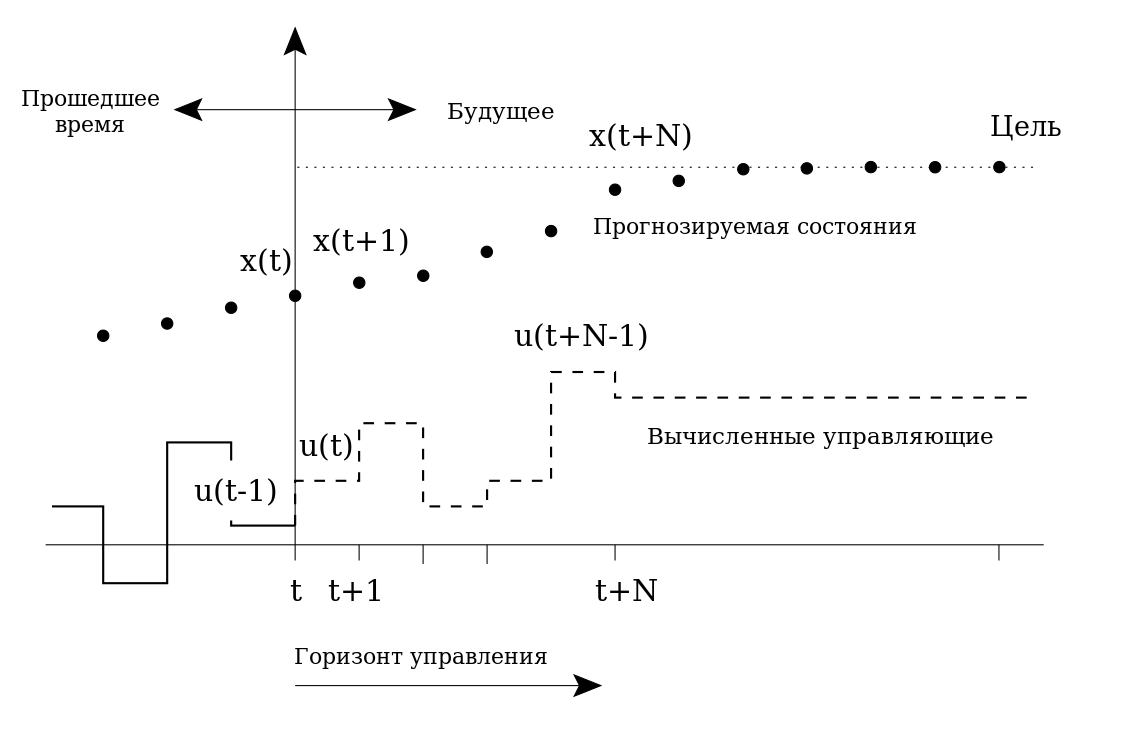
\includegraphics[width=\textwidth]{img/mpc_diag(1).png}
    \caption{Принцип работы модельного прогнозирующего управления}
    \label{fig:my_label}
\end{figure}

Тогда, модельный прогностический контроллер определяется:
\begin{enumerate}
    \item Целовой функционал, которой сведен к минимуму.
\item Внутренняя модель системы для прогнозирования поведения системы.
\item ограничения, которые должны быть удовлетворены.
\end{enumerate}
\newpage
И модельный прогностический регулятор работает в соответствии с следующем:
\begin{enumerate}[noitemsep]
    \item решить задачу оптимизации для вычисления минимума целевого функционала.
\item  Получить последовательность запланированных сигналов управления.
\item  Применить первый управляющий сигнал.
\item  Повторить процедуру планирования.
\end{enumerate}

\subsection{Модельное прогнозирующее управление на основе \\
обучения (Learning-based model predictive control)}
Традиционная модельного прогностического управления опирается на заданном динамическом модели системы и решает задачу оптимизации оптимального управления с ограничениями (уравнение 4,5,6,7).\\

Затем, если динамическая модель недоступна или не точна, эффективность модельного предсказательного регулятора модели будет затронута, и результаты не будут оптимальными.
Обучение может быть использовано для повышения эффективности моделного прогнозного управления, путем (1) обучения остаточной части в качестве коррекции модели, или (2) обучения всей модели на данных, собранных из взаимодействия на реальном управляющем объекте.\\

Мы заинтересованы во втором выборе (2), чтобы в полной мере использовать обучение.
Для того чтобы сформулировать обучающую систему модельного прогностического управления , мы должны выбрать (1) Как мы будем описать обучающей среды (2) Обучаемую модель (3) метод оптимизации. И потом формировать целый цикл управления.\\

В этой работе мы выбрали следующее:\\
(1) Мы определим среду как среду обучения с подкреплением (Марковский процесс принятия решений).\\
(2) Базовой моделью будет нейронная сеть, но чтобы справиться с неопределенностью в модели, мы попытаемся в будущем использовать ансамбль нейронных сетей.\\
(3) Поскольку информация о целевой функции системы непрактична для получения, мы будем использовать оптимизация без производных, в этой работе мы выбрали использовать оптимизатор максимизации перекрестной энтропии.


\newpage
\subsection{Обучения с подкреплением}
Обучение с подкреплением, идея которого была произведена от психологии, является подразделом машинного обучения, изучающим, как агент должен действовать в окружении, чтобы максимизировать некоторый долговременный выигрыш. 

\begin{figure}[H]
    \centering
    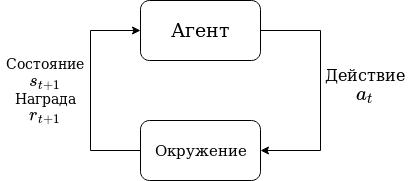
\includegraphics[height=5cm]{img/RL_ru.png}
    \caption{Обучение с подкреплением}
    \label{fig:my_label}
\end{figure}

Окружение обычно формулируется как марковский процесс принятия решений (МППР) с конечным множеством состояний, и в этом смысле алгоритмы обучения с подкреплением связаны с динамическим программированием. Вероятности выигрышей и перехода состояний в МППР обычно являются величинами случайными, но стационарными в рамках задачи.
\begin{center}
\captionof{figure}{марковский процесс принятия решений}
 \begin{tikzpicture}[->, >=stealth', auto, thick, node distance=3cm]

    \tikzstyle{round}=[thick,draw=black,circle]

    \node[round] (s0) {$s_0$};
    \node[round,right= 25mm of s0] (s1) {$s_1$};
    \node[round,above right=7mm and 10mm of s0] (a1){$a_1$};
    \node[round,right= 25mm of s1] (s2) {$s_2$};
    \node[round,above right=7mm and 10mm of s1] (a2){$a_2$};
    \node[round,above right=7mm and 10mm of s2] (a3){$a_3$};

    \path (s0) edge node[below] {$p(s_{t+1}|s_t,a_t)$}(s1)
          (s0) edge node {$\pi_\theta$} (a1)
          (a1) edge node {} (s1);
    \path (s1) edge node[below] {$p(s_{t+1}|s_t,a_t)$}(s2)
          (s1) edge node {$\pi_\theta$} (a2)
          (a2) edge node {} (s2);
    \path (s2) edge node {$\pi_\theta$} (a3);
\end{tikzpicture}
\end{center}
Где $s_t$ - состояние, $a_t$ действие, $r_t$ Награда  \\
Вероятность перехода : $p(s_{t+1}|s_t,a_t)$ \\
Функция стратегии: которая дает наилучшее действие для каждого состояния после процесса обучения: $a \sim \pi_\theta (a_t|s_t)$\\
Цель состоит в том, чтобы максимировать ожидаемые долгосрочные выгрриш:
$$J (\theta)=\sum_{t=1}^{T} \mathbb{E} [r (s_t), \theta]$$
\newpage
\subsection{Обучение с подкреплением для MPC}
Чтобы связать эту часть с формулировкой задачи оптимального управления (раздел 3.1), обучение подкреплению опирается на решение задачи оптимального управления бесконечным горизонтом (уравнения 6,7) путем оценки закона управления состоянии $u(t)=h(x(t))$ для измеренного вектора состояния $x(t)$ и применения вектора управления $u(t)$ к системе, после чего она измерит результирующий вектор состояния$x(t+1)$, оценив стоимость $r(s(t), u(t))$ и улучшив контроллер h на основе оценки. Это повторяется на каждом дискретном временном шаге t. Формально модель системы не требуется для обучения с подкреплением, но она может быть обучена, в этом случае она называется обучением с подкреплением на основе модели.\\
(в обучением с подкреплением мы используем $s$ вместо $x$, $a$ действие вместо $u$ управления, Стоимость будет называться наградой )\\

В обучением с подкреплением на основе модели мы рассматриваем динамическую систему, регулируется переходной функцией $f_\theta$, такой,что при текущем состоянии $s_t$ и текущем входе $a_t$ следующее состояние $s_{t+1}$ задается $s_{t+1}=f(s_t, a_t)$. Для вероятностной динамики (что имеет место для всех физических систем), условное распределение следующего состояния с учетом текущего состояния и действия как некоторого параметризованного распределений: $f_\theta(s_{t+1}|s_t , a_t)=p(s_{t+1}|s_t,a_t;\theta)$.\\
\begin{figure}[H]
    \centering
    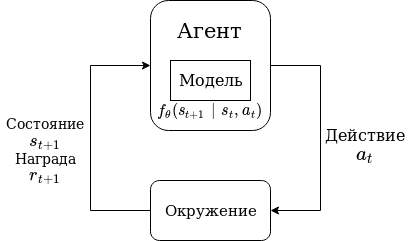
\includegraphics[height=5.5cm]{img/MBRL_ru.png}
    \caption{Обучение с подкреплением на основе модели}
    \label{fig:my_label}
\end{figure}
Таким образом, обучение прямой динамики является задачей подбора аппроксимации $\tilde{f}$ истинной переходной функции,учитывая измерения $\mathcal{D}=\{(s_n,a_n), s_{n+1}\}_{n=1}^N$ из реальной системы.\\

Обучившись динамическую модель $\tilde{f}$, мы можем использовать ее для прогнозирования распределения по траекториям состояний, возникающих в результате применения последовательности действий. Вычисляя ожидаемое вознаграждение по траекториям состояний, мы можем оценить несколько возможных последовательностей действий и выбрать оптимальную последовательность действий для использования.\\

\begin{algorithm}[H]
\SetAlgoLined
\DontPrintSemicolon
\caption{Обучение с подкреплением на основе модели}
Run a random policy;\\
Collect data $\mathcal{D}=\{(s_n,a_n), s_{n+1}\}_{n=1}^N$;\\
\For{number of iterations}{
compute the loss $\sum_i ||f_\theta(s_i,a_i)-s_{i+1}||$;\\
learn the dynamical model $f_\theta(s_t,a_t)$ by minimizing the loss;\\
\For{plan horizon}{
plan through  $f_\theta(s_t,a_t)$ to choose a sequence of actions $U^*(t)$;\\
execute the actions $U^*(t)$;\\
observe the resulting data $\{(s_t,a_t, s_{n+1})_j\}$;\\
append data $\{(s_t,a_t, s_{n+1})_j\}$ to $\mathcal{D}$;
}
}
\end{algorithm}

\subsection{Ансамбль нейронных сетей\\
Ensemble Neural Networks (ENN)}
В обучении c подкреплением на основе моделей мы должны выбрать класс моделей для прогнозирования динамики задачи (неизвестная динамическая функция). Этот выбор имеет решающее значение для алгоритмов обучения подкреплению на основе моделей, поскольку даже небольшое смещение может существенно повлиять на качество соответствующего контроллера.\\

Задача состоит в том, чтобы выбрать модель, которая может хорошо работать в режимах низких и высоких данных, т. е. на ранних стадиях обучения данные недостаточны, а высокоэкспрессивные аппроксиматоры функций могут быть переобучен. На более поздних стадиях обучения данные многочисленны, и в случае системы со сложной динамикой простые аппроксиматоры функций могут быть недостаточно недообучение.\\
\newpage
Нам нужна модель, которая может справиться с двумя типами неопределенности:
\begin{enumerate}
    \item Алеаторическая неопределенность; возникает из присущей системе стохастичности, например, шума наблюдения и шума процесса.
\item Эпистемическая неопределенность; соответствует субъективной неопределенности относительно функции динамики, из-за отсутствия достаточных данных, чтобы однозначно определить основную систему точно.
\end{enumerate}

Первый тип неопределенности может быть захвачен путем вывода параметров параметризованного распределения (математическое ожидание $\mu$ и ковариация $\Sigma$); для этого мы можем использовать параметризацию $\hat{p}_\theta(s'|s, a)=\mathcal{N}(\hat{f}_\theta(s,a),\Sigma)$.
Математическое ожидание $\hat{f}_\theta (s,a)$ задается нейронной сетью, и ковариация $\Sigma$ условного гауссовского распределения может быть обучена (или для простоты установить постоянное значение).\\

В случае бесконечных данных второй тип неопределенности исчезает, но для набора данных маленького размера эта неопределенность влияет на точность предсказания переходов. Простой и недорогой способ справиться с этой неопределенностью-использовать ансамбль нейронных сетей, которые аппроксимируют задний $p (\theta | \mathcal{D})$ с набором моделей $E$, каждая из которых имеет параметры $\theta_i$. 
В практике, с глубокими моделями нам нужно просто инициализировать параметры каждой модели $\theta_i$ с другой случайной инициализацией $\theta_i^0$ и использовать разные пакеты данных $D_i$ на каждом шаге обучения.

\begin{figure}[H]
    \centering
    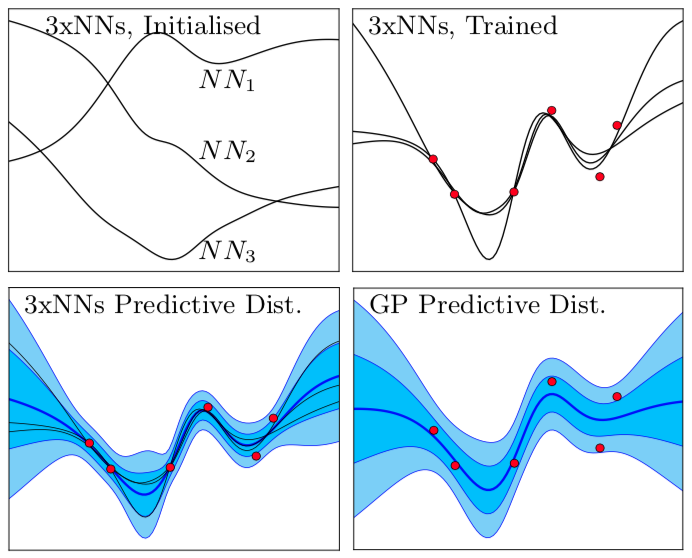
\includegraphics[height=6cm]{img/ensemble_intro.png}
    \caption{Предсказания неопределенности с ансамблю нейронных сетей}
    \label{fig:my_label}
\end{figure}

\begin{algorithm}[H]
\SetAlgoLined
\DontPrintSemicolon
\caption{Обучение с ансамблю нейронных сетей}
Initialize E neural network with different random initialization $\theta_i^0$;
Run a random policy;\\
Collect data $\mathcal{D}=\{(s_n,a_n), s_{n+1}\}_{n=1}^N$;\\
\For{number of iterations}{
collect $E$ datasets $\mathcal{D}_i$ N time (with replacement) from $\mathcal{D}$, $N=size(\mathcal{D})$;\\
train each of the E neural network using one of datasets $\mathcal{D}_i$\\
with loss $\sum_i ||(f_\theta)_i(s_i,a_i)-s_{i+1}||$;\\
\For{plan horizon}{
compute the predictive probability distribution
$$f_\theta(s_t,a_t)=\frac{1}{E}\sum_{i=1}^E (f_\theta)_i(s_t,a_t)$$\\
plan through  $f_\theta(s_t,a_t)$ to choose a sequence of actions $U^*(t)$;\\
execute the actions $U^*(t)$;\\
observe the resulting data $\{(s_t,a_t, s_{n+1})_j\}$;\\
append data $\{(s_t,a_t, s_{t+1})_j\}$ to $\mathcal{D}$;
}
}
\end{algorithm}

\subsection{Выборка траектории с использованием частиц}


\subsection{Максимизация перекрестной энтропии\\
Cross-Entropy maximization (CEM)}

\newpage
\subsection{Алгоритм}
\newpage
\subsection{Результаты и обсуждения}
\newpage
\section{Заключение}
В этой работе, согласно плану, мы закончили исследовательскую часть выпускникого проекта и приступили к экспериментальной части.\\

Работа по достижению этой части включала тщательное изучение всех упомянутых алгоритмов, написание кода для тестирования и исследование плюсов и минусов каждого из них. Эта работа также привела к публикации статьи о нашей работе с PILCO.
Обсуждая результаты нашей работы до сих пор, мы имеем четкое представление о различных алгоритмах обучения с подкреплением которые могут быть использованы для нашей задачи.\\

Безмодельные алгоритмы (например, SAC) могут быть использованы для изучения оптимальной политики для широкого круга задач, превосходящей производительность человека и классические управления после полного процесса обучения, но они страдают от проблемы неэффективности пробы, что делает их непрактичными для реальных приложений робототехники. \\

С другой стороны,алгоритмы обучения с подкреплением на основе модели изучают модель окружающей среды, а затем используют планирование в соответствии с изученной моделью. Это повышает эффективность пробы учебного процесса, но делает систему уязвимой к ошибкам модели, что приводит к плохой производительности или ограничению в работе (как в случае с PILCO).\\

Наша работа в следующем будет сосредоточена на попытке найти компромисс между алгоритмами без моделей и на основе моделей и использовать оптимальное управление наряду с обучением (learning-based control) для решения проблемы сборки.
\newpage
\begin{thebibliography}{9}
    \addcontentsline{toc}{section}{\refname}
    \bibitem{go} Silver, D., Huang, A., Maddison, C. J., Guez, A., Sifre, L., Van Den Driessche, G., ... & Dieleman, S. (2016). Mastering the game of Go with deep neural networks and tree search. nature, 529(7587), 484.
    \bibitem{TRPO}   J. Schulman, S. Levine, P. Moritz, M. I. Jordan, and P. Abbeel. “Trust region policy optimization”. In:CoRR, abs/1502.05477 (2015).
    \bibitem{openai_gym} G. Brockman, V. Cheung, L. Pettersson, J. Schneider, J. Schulman, J. Tang, and W. Zaremba. “OpenAI Gym”. In: arXiv preprint arXiv:1606.01540 (2016).
    \bibitem{Sutton} Richard S Sutton and Andrew G Barto. Reinforcementlearning: An introduction, volume 1. MIT press Cambridge, 1998.
    \bibitem {task} Зенкевич С. Л., Ющенко А. С. Основы управления манипуляционными роботамиб Изд-во МГТУ им. Н. Э. Баумана, 2004
    \bibitem{survey} Deisenroth M.P., Neumann G., Peters J. A survey on policy search for robotics Found. Trends Robot., 2 (1–2) (2013), pp. 1-142
    \bibitem{data-efficient} Konstantinos Chatzilygeroudis, Roberto Rama, Rituraj Kaushik, Dorian Goepp, Vassilis Vassiliades, et al.. Black-Box Data-efficient Policy Search for Robotics. IEEE/RSJ International Conference on Intelligent Robots and Systems (IROS), Sep 2017, Vancouver, Canada

\end{thebibliography}

\end{document}

\usepackage[english,russian]{babel}